\documentclass[conference]{IEEEtran}
\pdfpagewidth=8.5in
\pdfpageheight=11in
%\usepackage{subfig}
\usepackage{subfigure}
\usepackage[pdftex]{}
\usepackage{todonotes}
\usepackage{listings}
\lstset {% general command to set parameter(s)
         language=C,
     basicstyle=\footnotesize,               % print whole listing small
%     keywordstyle=\color{black}\bfseries, % underlined bold black keywords
%     identifierstyle =\color{black},  % nothing happens
%     commentstyle=\color{black}\emph, % white comments
     %stringstyle=\ttfamily,          % typewriter type for strings
%     stringstyle=\color{black},       % typewriter type for strings
         tabsize=4,
         showtabs=false,
     showstringspaces=false}
%can't figure this one out for particles bandwidth
%\usepackage[caption,label]{subfig}

%\newcommand{\TITLE}{D\textsuperscript{\huge{2}}T: Doubly Distributed Transactions for High Performance and Distributed Computing}

\newcommand{\DDT}{D\textsuperscript{2}T~}
\newcommand{\DDTns}{D\textsuperscript{2}T}

\hyphenation{sub-trans-ac-tion}

\addtolength{\parskip}{-0.04in}

% in order for balance columns to work, it has to be before begin document...
%\balancecolumns

\begin{document}

%\conferenceinfo{MSST'14,} {November 17, 2013, Denver, Colorado, USA.}
%\CopyrightYear{2014}
%\crdata{978-1-4503-1103-8/11/11}
%\clubpenalty=10000
%\widowpenalty = 10000

\title{Consistency and Fault Tolerance Considerations for the Next Iteration of the DOE Fast Forward Storage and IO Project}

\author{
\IEEEauthorblockN{Jay Lofstead}
\IEEEauthorblockA{Sandia National Laboratories\\gflofst@sandia.gov}
\and
\IEEEauthorblockN{Ivo Jimenez}
\IEEEauthorblockA{University of California, Santa Cruz\\ivo@cs.ucsc.edu}
\and
\IEEEauthorblockN{Carlos Maltzahn}
\IEEEauthorblockA{University of California, Santa Cruz\\carlosm@soe.ucsc.edu}
}
\maketitle

\begin{abstract}
With phase 1 of the Fast Forward Storage and IO Stack project complete, it is
an excellent opportunity to evaluate many of the decisions made to feed into
the phase 2 effort. The initial effort to define a next generation file system
has made admirable contributions in architecture and design. Formalizing the
general idea of data staging as burst buffers for the file system will help
manage the performance variability and offer the data processing opportunities
outside the main compute and file system. Adding a transactional mechanism to
manage faults and data visibility helps enable effective analytics without
having to work around the IO stack semantics.

While these and their other contributions are valuable, similar efforts made
elsewhere may offer attractive alternatives or differing semantics that could
yield a more feature rich environment with little to no additional overhead.
For example, the Doubly Distributed Transactions (\DDTns) protocol offers an
alternative approach for incorporating transactional semantics into the data
path. The PreDatA project examined how to get the best throughput for data
operators can offer some insights for refining the Burst Buffer concept.

This paper examines some of the choices made by the FastForward team and
compares them with other options and offers observations and suggestions based
on these other efforts.  This will include some non-core contributions of other
projects, such as some of the demonstration metadata and data storage
components generated while implementing \DDTns, to make suggestions that may
help the next generation design for how the IO stack works as a whole.

\end{abstract}

%\category{D.4}{Software}{Operating Systems}
%\category{D.4.7}{Operating Systems}{Organization and Design}[hierarchical design]

%\terms{Design, Performance}

\section{Introduction}

Current production HPC IO stack design is unlikely to offer sufficient features
and performance to adequately serve the needs of an extreme scale platform. To
address these limitations, a joint effort between the US Department of Energy's
Office of Advanced Simulation and Computing and Advanced Scientific Computing
Research commissioned an effort to develop a design and prototype for an IO
stack suitable for the extreme scale environment. This is a joint effort led by
Lawrence Livermore National Laboratory, with the DOE Data Management Nexus
leads Rob Ross and Gary Grider as coordinators and contract lead Mark Gary. The
participating labs are LLNL, SNL, LANL, ORNL, PNL, LBNL, and ANL. Additional
industrial partners contracted include the Intel Lustre team, EMC, DDN, and the
HDF Group. This team has developed a specification
set~\cite{fastforward:2014:docs} for a future IO stack to address the
identified challenges. The first phase recently completed with a second phase
getting underway. The core focus of the first phase was basic functionality and
design. Overriding many of the decisions during this and any subsequent phases
is the reality of budgets. Placing GBs of NVRAM on every node, while a
potentially advantageous approach, is not financially feasible. With this in
mind, the second phase will refine this design incorporating fault recovery and
other features missing from the first phase.

The overall design seeks to offer a byte-granular, multi-version concurrency
control. Through the use of a copy-on-write style mechanism, multiple versions
of a file can be stored in potentially greatly reduced space. It assumes the
client interface will be through an IO library affording a more complicated
interface that offers richer functionality without requiring user code changes.
Managing most data access in a machine-local layer rather than requiring
writing to centralized storage will better support the performance and energy
requirements of extreme scale integrated application workflows. At a more
detailed view, the various layers of the IO stack each contribute different
functionality and performance implications.

The basic architecture incorporates five layers. The top layer is a high level
IO library, such as the demonstration HDF-5 library. The intent is to only have
access to the storage stack through such an API to manage the complexity of
working with the lower layers. Below the user API is an IO forwarding layer
that redirects IO calls from the compute nodes to the IO dispatching layer.
This IO forwarding layer is analogous to the function of the IO nodes in a
BlueGene machine. The next two layers have considerable functionality. The IO
dispatcher (IOD) serves as the primary storage interface for the IO stack and
is the only way to reach the persistent storage array in lower layers. The
Data Access Object Storage (DAOS) layer serves as the persistent storage
interface. At the bottom is the Versioning Object Storage Device (VOSD). It
serves as the interface for storing objects of all types efficiently.

The focus of this paper is primarily the IOD layer given the critical role it
has in the performance and functionality of the entire stack. Most of the key
features explored in this paper all have a strong presence in the IOD layer
motivating the focus of this examination.

The core idea for IOD is to provide a way to manage the IO load that is
separate from the compute nodes and the storage array. Communication intensive
activities, such as data rearrangement, can be moved to the IOD layer
offloading the communication load from the compute nodes. IOD has three main
purposes. First, if the optional burst buffer is available, it works as a fast
cache absorbing write operations for the slower trickle out to the central
storage array. It can also be used to retrieve objects from the central storage
array for more efficient read operations and offers data filtering to make
client reads more efficient.  Second, it offers the transaction mechanism for
controlling data set visibility and to manage faults that would prevent a data
set from being used. Third, data processing operations can be placed in the
IOD. These operations are intended to offer data rearrangement, filtering, and
similar operations prior to data reaching the central storage array.

While these ideas are not necessarily new, they are new twists on best of class
efforts for these technologies. For example, offloading the collective
two-phase data sieving from the compute nodes to reorganize data has proven
effective at reducing the total time for writing data due to fewer participants
involved in the communication patterns~\cite{lofstead:2011:nessie-staging}.
Beyond these broad items, there are many important details some of which are
examined in more detail below.

Along with the analysis of the published design documents, a discussion of the
design philosophy representing the overall intent is presented. This
information represents information that may or may not have been written down,
but is the intent of ultimate product. These insights were gained based on
personal conversations with the team members discussing some of the potential
challenges with the design as written. These ideas are presented to give a
fuller picture of where the project is going rather than dwelling on the
limitations of the published documents.

The rest of the paper is organized as follows. Section~\ref{sec:burst}
discusses some of the features of incorporating burst buffers as designed and
suggests some considerations and alternatives for the next generation of this
project. Section~\ref{sec:transactions} discusses the transactions approach
offered in the IOD layer and the corresponding epochs in the DAOS layer. It
also offers a comparison to the \DDT system given the very similar high-level
design and motivating use case.  Section~\ref{sec:summary} discusses the system
overall with recommendations on what design elements should be considered based
on broader issues with current HPC data centers. The paper is concluded in
Section~\ref{sec:conclusion} with a summary of the broad issues covered in the
paper.

\section{Burst Buffers}
\label{sec:burst}

The idea of burst buffers were initially explored in the context of data
staging~\cite{abbasi:2007:datatap,Abbasi:2009:datatap,nisar:2008:staging,zheng:2010:predata}.
These initial designs all use extra compute nodes to represent the data storage
buffer given the lack of any dedicated hardware support for this functionality.
The desired outcome of these initial studies is to motivate how such
functionality might be incorporated and the potential benefits.  Later, these
concepts were proposed to be incorporated as part of the IO
stack~\cite{bent:2012:challenges,bent:2012:burst-buffer}.  The current
FastForward IOD design recommends incorporating SSDs, but specifically lists
these devices as optional. Unfortunately, both incorporating burst buffers and
the use of SSDs in the IOD layer may be problematic.  First, the IOD and DAOS
designs currently are written assuming burst buffers. This means that the
bulk of IO operations will only hit the IOD layer and proposed functionality,
such as the function operators, do not discuss the impact on the DAOS layer or
the operators themselves should a burst buffer not be available.  Consider the
important functionality of data rearrangement and doing things like changing
the fast array dimension on shared, spinning media.  The design of DAOS assumes
that it will only be involved when persisting a completed transaction and only
for a fraction of the total transactions created. 

One of the bigger concerns is the observation that the original data staging
proposals all used compute nodes while the newer proposals seek not only to
make them a fixed portion of the IO stack, but also shared across all machine
users. The PreDatA~\cite{zheng:2010:predata} paper in particular examines the
potential costs and advantages of where to place operators similar to the IOD
proposed function shipping. There are two key takeaways from PreDatA. First,
placement matters.  Depending on the communication intensity vs. computation
intensity, where along the IO path to place the operation can matter
significantly. Second, and more importantly, the amount of time spent
processing for the operators was stretched to the point where it consumed
nearly all of the time between IO operations. The given ratios of compute
processes to staging process examined is representative for future extreme
scale platforms. If anything, the ratios offer more staging processes than IOD
processes would be available.

In the case of the written IOD design, it describes a fixed-sized staging area
shared across all users simultaneously.  This is unlikely to be useful because
of the limited compute and communication capacity to spare to perform these
operations at a bottleneck in the IO path.  The use of a separate data staging
area intentionally separate from the IO path allows using operators on limited
resources leaving the IO path clear for strictly data movement. A nuance of
this design is discussed in the Design Philosophy below.

By concentrating this functionality into the storage stack, three problems
arise.  First, the amount of network bandwidth, IO bandwidth, and compute power
consumed for example operations from a single application is likely to
completely monopolize the IOD processes. Second, if space and time partitioning
is used instead, the functionality risks being too small to be useful. Third,
the hardware performance advantage for SSDs is questionable. Current NAND-based
flash devices top out at around 400 MB/sec. The key spec that is missing from
this number is that 400 MB/sec is a measure of the fixed number of available
IOPS multiplied by the block size. This represents the ideal streaming
performance possible. The problem is that it costs an IOP to read 1 byte or 1
block (4KB or 8KB, depending on the device). It costs 1 IOP to write a full
block--usually. In some cases, it will cost 2 IOPs.  This accounts for the
required pre-erase write prior to writing to a reused block. In the worst case,
it can be 3 IOPS per write. This would be for a partial block write (read the
old block, erase, write the modified block). One-third of 400 MB/sec, about 133
MB/sec, is well below the streaming performance of HDDs.  Granted, there is
still rotational and seek latency to deal with for HDDs, but the advantage for
SSDs has evaporated and potentially turned into a penalty at a considerable
cost premium.  There are faster SSD solutions on the market that incorporate
DRAM for caching and using the PCIe bus, for example, but their price precludes
them from use in an extreme scale platform.

Given these features, the optionality and even incorporation of burst buffers
in the current design should be carefully considered. Much of the advanced, key
functionality proposed as they are currently designed ultimately relies on the
existence of burst buffers to work. Further thought about how to have an IOD
layer both with and without a burst buffer is required before they can be
considered optional. As the design stands today, they are a required part of
the IOD layer for proper functioning. Unfortunately, it is not clear that they
can address the performance concerns they are intended to cover.

\subsection{Design Philosophy}
The burst buffers design, as presented in the IOD documents, limits the
placement of the function operators and SSDs for buffers to the IO nodes. The
team does acknowledge the limitations of this design and intend to ultimately
focus on spreading the IOD layer from the IO nodes into the compute area as
well.  This is intended both to help address the limitations of the IO
bandwidth and compute capability of these few nodes for data processing, but
also to take advantage of new layers in the storage hierarchy. By incorporating
NVRAM into compute nodes, new options for buffering data prior to being moved
to centralized storage become available and addresses some of the concerns
about SSD performance. This lessens the impact of some operators while offering
additional options for places to store data.

Burst buffers being optional is a high level goal, but not one considered at a
detailed level with the design. For example, if there is no burst buffer, all
of the advanced functionality proposed for the IOD layer would have to work
against the DAOS layer instead. For example, function shipping assumes it will
operate on fast, local data within the IOD layer rather than against the
globally shared DAOS layer. With the additional desire to support using compute
node resources for these operations, serious work will be required to make a
fully functional end-to-end IOD layer implementation for a production system.

Another concern that is acknowledged, but no thought has been applied to is the
requirement that a single IOD process be the master for any operation. Should
the number of concurrent applications exceed the available nodes, sharing an
IOD process will be required. Since partitioning of the IOD processes for
exclusive use by particular applications is the assumed operating mode, should
insufficient IOD resources be available, either a job could be delayed or IOD
resources could be reallocated from a different process could be redeployed for
use by the new job. These sorts of considerations still need to be made for a
full production system.

\section{Transactions and Epochs}
\label{sec:transactions}

The transaction mechanism manifests in two forms. At the IOD layer, they are
called transactions and are used to judge whether or not an output is complete
or not and control access through treating the transaction ID as a version
identifier. At the DAOS layer, they are called epochs and represent persisted
(durable) transactions from the IOD layer. Each of these offers different
functionality, but are connected as is explained below. How these differ from
the \DDT approach is also explored. While IOD's and \DDTns's transactions are
seemingly very different, they use a similar high-level design, but very
different implementation, to solve the same problem.

\subsection{IOD Transactions}
To understand how transactions are used in the IOD layer, some terminology and
concepts must be explained first. At the coarsest grain level is a container.
Each container serves to host a transaction and contains a collection of
objects. Conceptually, containers corresponds to a file in a traditional file
system. The objects in each container represent different data within a file.
The three initially defined object types are key-value store, array, and blob.
The easiest way to understand these types is to evaluate these from the
perspective of an HDF-5 file, the initial user interface layer. The key-value
store represents a collection of attributes or groups. The array represents
part of a potentially multi-dimensional array. It is referred to as
a shard because it is likely a small piece of a globally defined array. The
blob represents a byte stream of arbitrary contents.  The fundamental
difference between an array and a blob is that the array has metadata
identifying its portion within the global, logical space while the blob is
simply a 1-dimensional array of bytes that is not shared across IOD nodes.
Should an operation be deployed into IOD to manipulate an array within a
container, it would operate on the array rather than on blobs. Given this
context, the transactions come in two forms.

First is a single leader transaction where the IOD manages based on calls from
a single client. The underlying assumption is that the client side will manage
the transactional operations itself and the single client is capable of
reporting to the IOD how to evolve the transaction state. 

The second form is called multi-leader and has the IOD layer manage the
transactions. In this case, when the transaction is created, a count of clients
is provided to the IOD layer. As clients commit their changes to the container,
the reference count is reduced. Once the count reaches 0, the transaction is
automatically committed.

\subsubsection{Design Philosophy}
Undocumented, but inherent in the design of these transactions is how faults
are detected. The initial design assumes the current Lustre fault detection
mechanism that can determine if a process or node is no longer reachable. This
defines how a fault will be detected and what will trigger a passive fault
recovery (i.e., transaction abort).

The team uses the term ``Primary'' to define the process(es) that contact the
IOD layer directly to open a container. Unfortunately, this term is never used
nor defined within any of the published documents. There are some very positive
and negative performance implications of this approach. On the positive side,
like PVFS, it is possible for a single process to open a container and share
that handle with other processes reducing the load on the IOD layer. The key
idea is that the single leader vs. multi-leader transaction mode is
automatically defined based on the number of Primary processes that start a
transaction on a container. This greatly simplifies any additional client-side
load in using the different styles of transactions. Also on the positive side,
it offers the ability to have a subset of processes that are considered
transaction participants affording reduced load on the IOD processes and more
localized transaction management on the client side. On the negative side, for
a fully IOD managed transaction, ALL processes must start the transaction on
the container forcing a potentially immense number of simultaneous calls to the
IOD layer to open a container. This sort of onslaught is what is dealt with on
metadata servers today with mass file opens. The reality is that this ends up
having the same sort of performance implications as distributed denial of
service attacks on the IOD processes.

Ultimately, with the passive detection of faults for Primaries, the transaction
mechanism can work very well. A mostly unstated restriction that is being
relaxed is that every sequential transaction on a container is considered
dependent on the earlier transaction. Should one output be delayed and the
subsequent five succeed, when the delayed process finally fails, all six
transactions are rolled back. The thought of using this mechanism to store
subsequent checkpoint outputs in the same container to both save space, but not
care if one fails, cannot work in the current form. This has been acknowledged
and is planned on being relaxed in phase two.

\subsection{DAOS Epochs}
The Epoch mechanism differs from transactions. Instead of focusing on when a
particular output is complete, an epoch represents incremental persisted copies
of a container. To simplify the mapping between an IOD transaction and the DAOS
epochs, when an IOD transaction is persisted to DAOS, the IOD transaction ID is
the used as the epoch ID. The key difference is that at the DAOS layer, some
transaction (epoch) IDs will not be represented.

\subsection{Metadata Management}
Eliminating metadata management as a special case and instead treating it just
as data is a central design goal of the Fast Forward project. This is a hybrid
approach to metadata management that is half-way between providing no inherent
metadata support and having a fully integrated, but separate metadata
manaegement system.

Eliminating metadata as a core component of a file system is not new. It has
been explored as part of the Light Weight File Systems
project~\cite{oldfield:lwfs}. In LWFS, the metadata service is explicitly
limited to a user task with the storage layer limited to data
storage/retrieval, authorization, and authentication. This approach proved
workable. Using this hybrid approach is less common~\cite{weil:2006:ceph} and
introduces other issues.

IOD and DAOS both share a philosophy that they will have to maintain the
metadata about how objects are striped and where they are placed. It was
decided that the additional data to track the namespace as well was a small
enough additional increment that it was worth maintaining within the system.

\subsubsection{Design Philosophy}
While the metadata design is not fully defined, there are a few things that
are intended. For example, there is a standard, well-known container that is
the system metadata. This includes the list of all other containers. This
container is treated like any other data in the system and striped as
appropriate at both the IOD and the DAOS layers. Unfortunately, this still
couples the metadata to a single object that must serialize access. If the
metadata, including information about striping and other data layout operations
were separated completely from the data path, more scalable throughput could be
achieved. The real challenge of this is introduced by the IOD, DAOS, and VOSD
layers. Each of these requires some different metadata storage and the
migration is transparent to the user. Supporting fully independent metadata
with this model is difficult. Serious thought on how to do this effectively
outside the data path should be considered for phase two.

Based on the lessons from the \DDT metadata
service~\cite{lofstead:2012:txn-metadata} construction and the prior
experiments with LWFS, having a completely separate metadata service is
workable. Rather than making it a bottleneck in the IO path, it is another
service that users must interact with if they need those services.  Users can
manage everything by maintaining the metadata including the list of objects
themselves. However, there are drawbacks to this 100\% client-side approach.

With a client-side only approach, there is a serious risk of the metadata
service and the object store getting out of sync.  While having a metadata-less
object storage service is desirable, the different semantics from traditional
file systems requires some considerations. In this case, should these services
get out of sync, three particular risks are introduced.  First, a client could
create an entry in the metadata service that does not correspond to any objects
in the object store. Second, a client could create objects that have no
associated metadata entries. Third, updates to the metadata or object store
service should be an atomic operation, but due to a lack of coordination, a
window where the system is inconsistent appears.

Ultimately, the consistency semantics required must be determined. If a
metadata service is required and it must be in sync with the object storage
service, then additional work must be performed. In traditional file systems,
the metadata and object storage updates are atomic. With decoupling metadata
from object storage, should this atomicity still be desired, it requires both
the ability for the services to participate in a task that is part of a larger
atomic operation and a higher-level mechanism to manage the atomic operation.

Overall, while additional work is required to maintain a client-side only
metadata service, it eliminates any potential bottlenecks related to updating
metadata related to the object storage. The burden of tracking striping and
other metadata that has traditionally been part of the metadata associated with
the file system will have to be maintained by the object storage service. The
lack of a centralized, serialized bottleneck to store that information improves
concurrency.

\subsection{Comparison to \DDTns}
The \DDT project~\cite{lofstead:2012:txn} sought to develop an efficient
approach for handling ACID-style transactions in an environment with parallel
clients and multiple servers (doubly distributed). Rather than being aimed
solely at data movement operations, \DDT seeks to address the general problem
of managing any operation with multiple clients and servers.  Consider the
management of the analysis/visualization area, potentially similar to the IOD
concept. The transaction protocol is used to help manage resizing of the
resource allocation to the various analysis and visualization components.  For
the purposes of this discussion, \DDT could also be used to manage changing how
IOD processes and/or nodes are used without exposing these changes to the
client processes prematurely.  This has been described and analyzed
previously~\cite{dayal:2013:io-containers}.

The example metadata and data storage services created as part of the \DDT
project have no dependencies between transactions that prevent visibility
should an older version be incomplete. This additional, intentional requirement
by IOD offers different functionality than \DDTns's example services. In the
case of \DDTns, the functionality is more minimal, but also avoids some of the
concerns outlined below.

The second iteration of the protocol~\cite{lofstead:2013:pdsw-txn} fixed
scalability issues and demonstrated a scalable client-side coordination model
with excellent performance. The performance measured for a complex transaction
with \DDT is illustrated in Figure~\ref{fig:performance}. This performance is
explored in detail in a previous paper~\cite{lofstead:2013:pdsw-txn}. The
breakdown of the number of participants in each role is shown in
Table~\ref{tab:scaling}. For comparison, consider the Number of
Sub-Coordinators equivalent to IOD processes. The Processes Per Sub-Coordinator
represents the number of clients that use a particular IOD process. For these
tests, we maintained a balanced distribution and always used at least two
sub-coordinators to slow down the processing.

\begin{figure}[ht]
%\vspace{-0.15in}
\centering
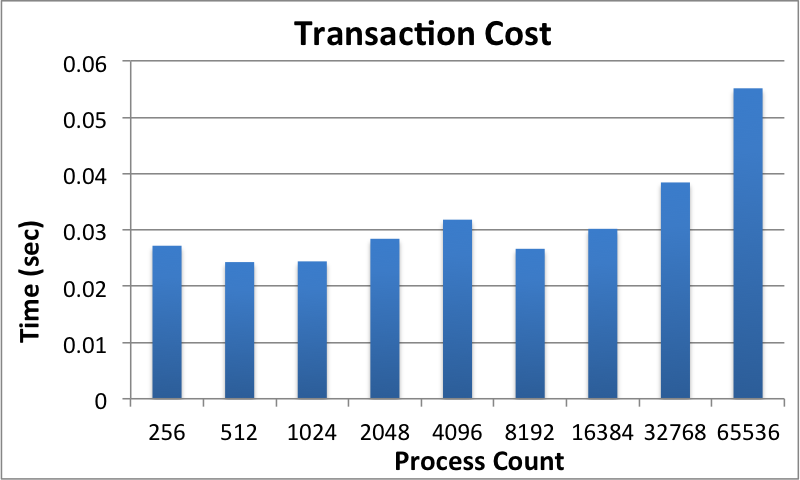
\includegraphics[keepaspectratio=true, width=0.9\columnwidth]{images/performance}
\vspace{-0.15in}
\caption{Total Transaction Overhead}
\label{fig:performance}
%\vspace{-0.15in}
\end{figure}

\begin{table}[ht]
    \vspace{-0.15in}
    \centering
    \caption[Scaling Configuration]{Performance Tests Scaling Configuration}
    \bigskip
    \vspace{-0.15in}

    \begin{tabular}{|r|r|r|}
\hline
Processes & \vtop{\hbox{\strut Number of}\hbox{\strut Sub-Coordinators}} & \vtop{\hbox{\strut Processes Per} \hbox{\strut Sub-Coordinator}}\\
\hline
%8 & 2 & 4 \\
%16 & 2 & 8 \\
%32 & 2 & 16 \\
%64 & 2 & 32 \\
%128 & 2 & 64 \\
256 & 2 & 128 \\
512 & 2 & 256 \\
1024 & 4 & 256 \\
2048 & 8 & 256 \\
4096 & 16 & 256 \\
8192 & 32 & 256 \\
16384 & 64 & 256 \\
32768 & 128 & 256 \\
65536 & 256 & 256 \\
\hline
    \end{tabular}
    \label{tab:scaling}
\end{table}

At a high level, both \DDT and the IOD transactions have the same design. In
both cases, a hierarchical model is employed. In the case of \DDTns, it is a
purely client-side tree using semi-synchronous messaging. The messaging itself,
in the current implementation, uses asynchronous MPI messages. The synchronous
component comes from the timeout mechanism used to detect faults.  It forces a
level of coordination and synchronization for the protocol. For IOD, it is a
server-side tree and fully asynchronous relying on the existing Lustre fault
detection mechanism for failure detection. In both cases, there is a master in
charge of managing the transaction and a collection of workers that aggregate
into the master through second-level leaders. Beyond that, there are some
significant differences. Some of the different choices made by IOD raise some
possible concern.

In the multi-leader model, using a count of client connections to determine if
transaction is complete is problematic. First, the aggregation of completion
messages are based on the local aggregation point reporting to the transaction
leader.  There is no ability to detect or recover from a failure of this IOD
process that would report to the transaction leader. The current assumption
that the IOD layer will be an MPI program is not workable until MPI can fully
support fault detection and recovery including removing and adding processes.
Second, since the counts represent a begin/end transaction pair, it suffers
from a lack of accountability for missing object (shard) writes. All it would
indicate is that a process started and ended a transaction connection. There is
no validation that a process has done everything required of it.

\begin{figure}[ht]
\centering
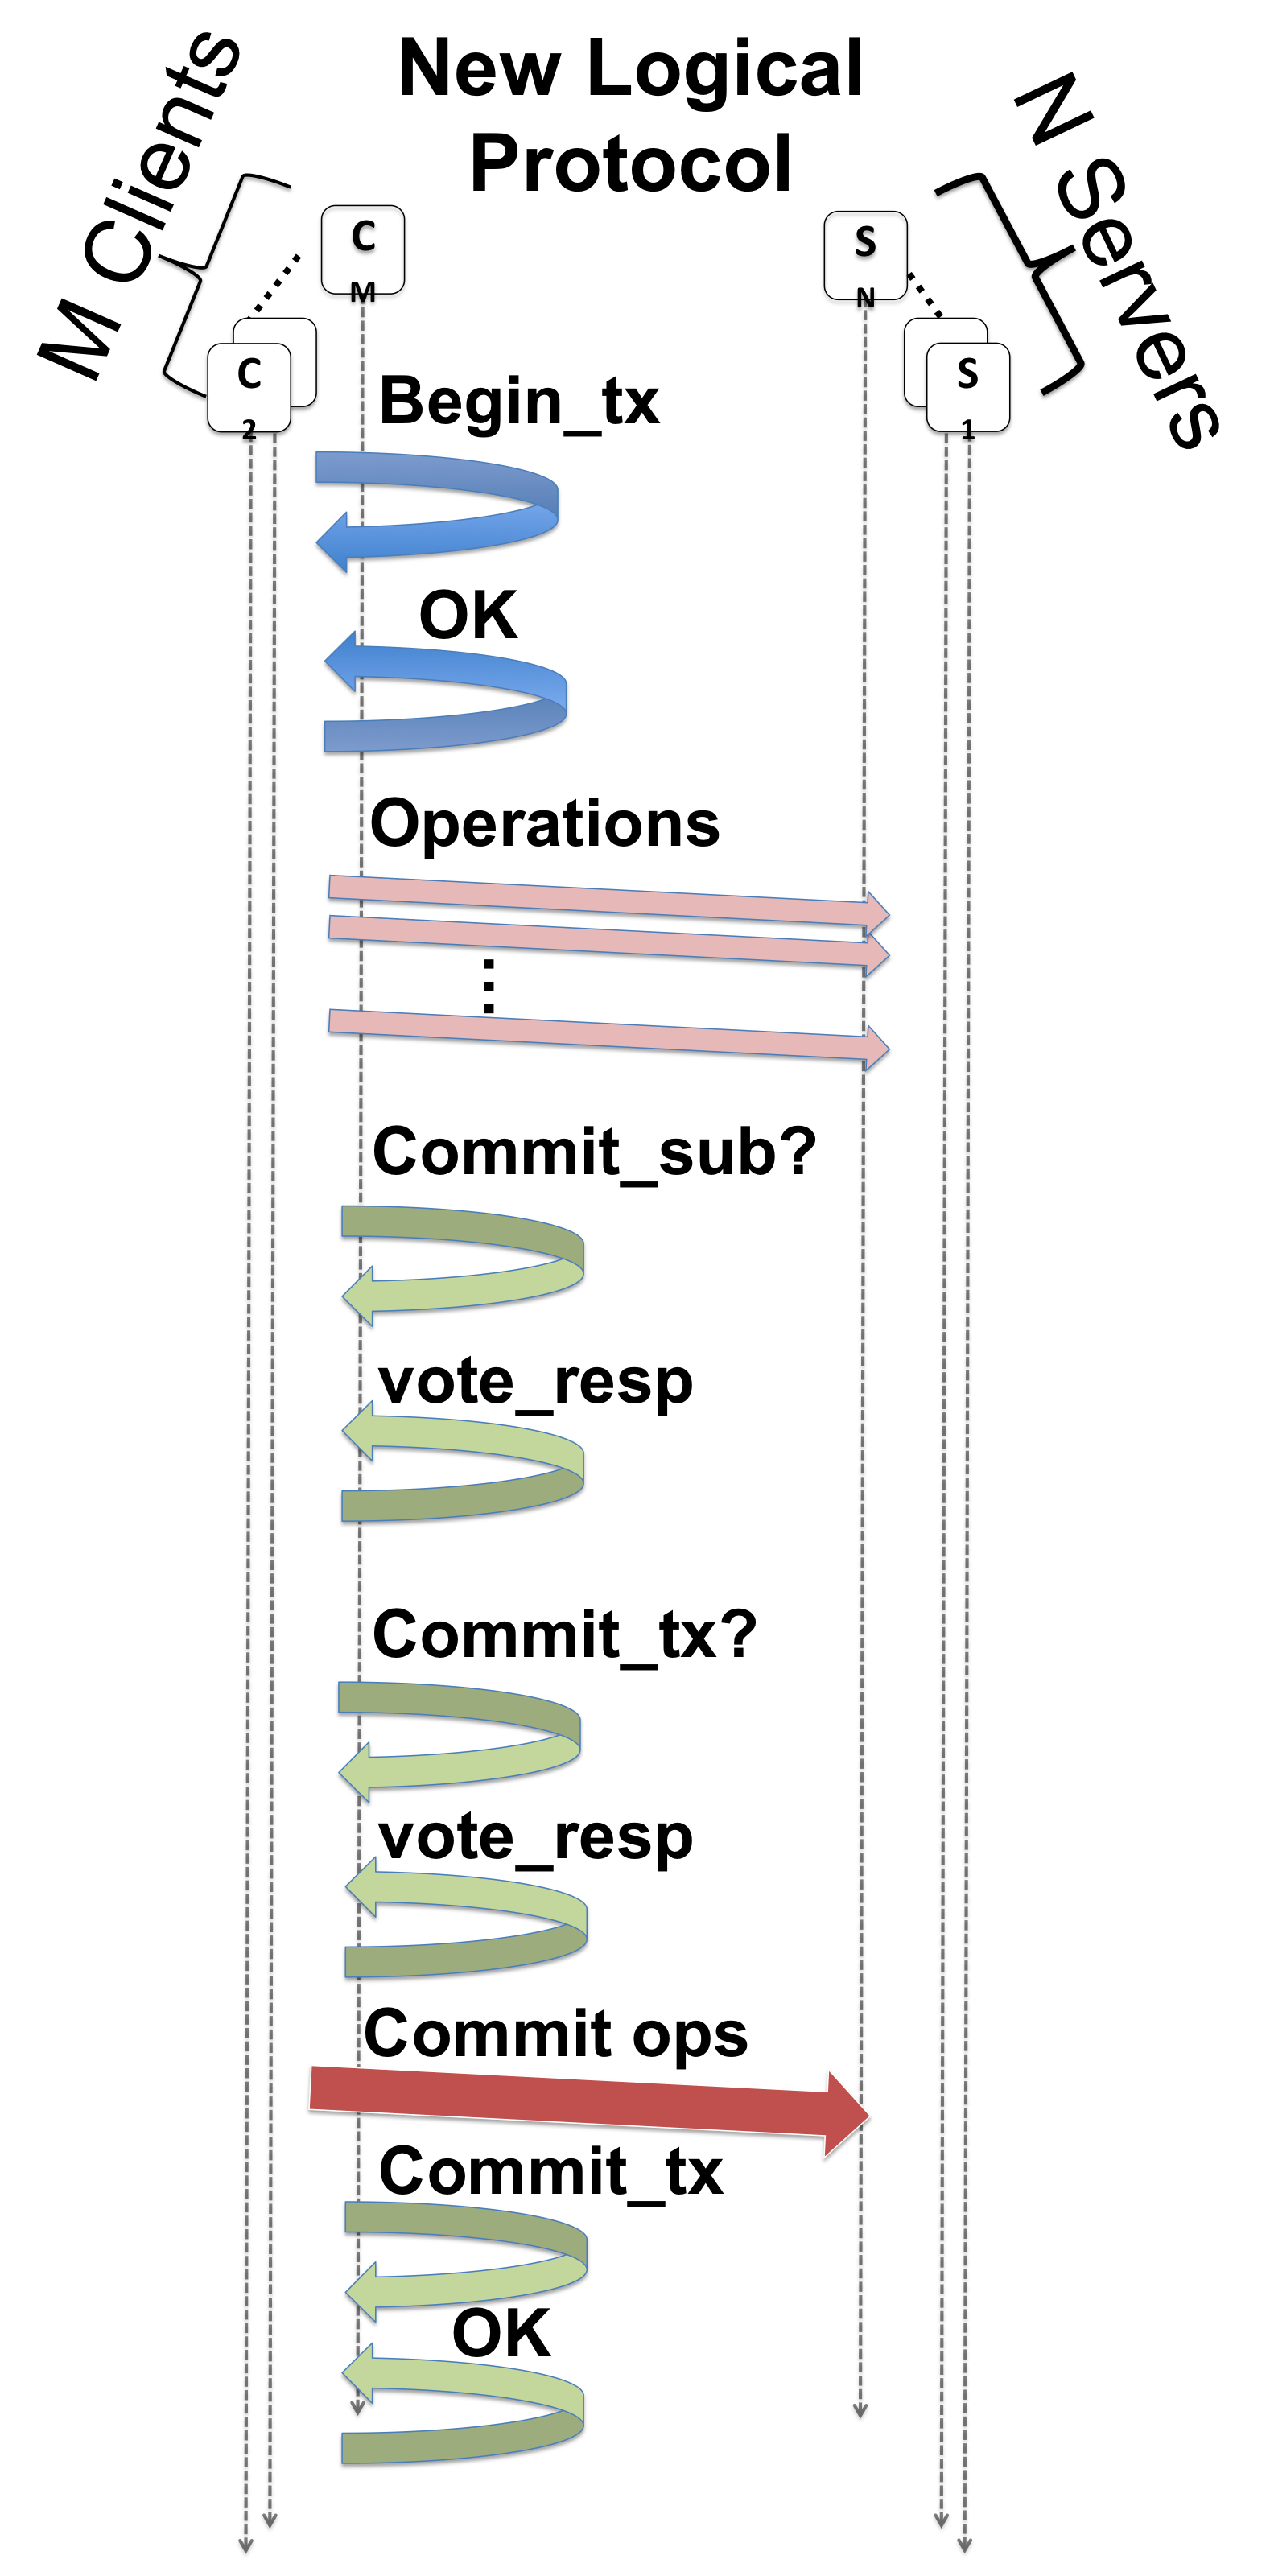
\includegraphics[keepaspectratio=true, width=0.9\columnwidth]{images/optimized-protocol}
\vspace{-0.15in}
\caption{Optimized Protocol}
\label{fig:optimized-protocol}
%\vspace{-0.25in}
\end{figure}

\DDT has addressed theses issues in a couple of ways. First, the
sub-coordinators each have a list of processes from which they expect messages.
Should a message be missed, it is noticed and corrective action can be taken.
Second, \DDT has the concept of sub-transactions. The messaging requirements
are illustrated in Figure~\ref{fig:optimized-protocol}.  Sub-transactions
represent finer grained operations than the entire output, \DDT can manage
multiple writes per client by using a sub-transaction to represent the output
for any item to the file (container). Because of how the sub-transactions are
managed, the singleton sub-transactions, ones in which only a single process
participates, must be declared before the transaction begins so that its
existence can be broadcast as part of the begin transaction message. This
ensures there is global knowledge that the sub-transaction is expected.  That
way if the coordinator (transaction leader) fails, whichever process takes over
that role knows to expect a completion message for that sub-transaction or the
overall transaction cannot complete. Global sub-transactions can be defined at
any time since they are a global, synchronized operation broadcasting their
existence. While this additional layer does introduce messaging, the overhead
is quite small.

The advantages of eliminating these messages is not performance as demonstrated
by the performance of \DDTns. Instead, it offers a much less synchronous model
that matches with different programming models, such as Charm++ or other
task-based approaches. Since it can work for the bulk-synchronous model also,
it is a more broadly applicable approach. This assumes that the observed
potential issues can be addressed successfully.

%\subsection{Comparison to Other Protocols}
%Alternatives, such as Paxos~\cite{Lamport:1998:paxos} algorithms like
%ZooKeeper~\cite{Hunt:2010:zookeeper}, suffer from two limitations making them
%unsuitable for this environment. First, the distributed servers in Paxos
%systems are all distributed copies of each other that eventually become
%consistent. Given the scale we wish to address, a single node's memory is
%unlikely to be able to hold all of the data necessary for many operations at
%scale. They also do not have a guarantee for when consensus will be achieved
%without using slower synchronous calls. For the tight timing we wish to
%support, we need guarantees of when a consistent state has been achieved.
%Second, these systems also all assume that updates are initiated from a single
%client process rather than a parallel set of processes as is the standard in
%HPC environments.
%
%\DDT uses a second layer of coordination on the client side that greatly
%increases the scalability by consolidating messages from clients into unique
%sets prior to sending to the overall coordinator. A gossip
%protocol~\cite{ganesh:2003:gossip-protocols} may appear sufficient for this
%purpose, but the delay of eventual consistency is strictly avoided with this
%protocol to ensure guarantees at particular states in the code. For example, if
%a failure occurs, the global understanding of the role of all processes is
%required in order for effective communication to occur for operations like
%creating sub-transactions or voting. In this case, the protocol can offer
%stronger statements about consistency than these protocols offer.  These
%features offer a way to easily scale the transaction protocol given the
%guarantees we wish to offer. The IOD approach does nothing to address these
%concerns.
%
%Another effort to offer consistency and data integrity for the ZFS file
%system~\cite{zhang:2010:zfs} covers some of the same territory. Instead of a
%focus on the processes all having a notion of completion as a transaction, this
%work focuses on the integrity of the data movement operations. We view this
%work as something that should be considered hand-in-hand with a transaction
%approach to ensure the integrity of the movement of the data in addition to the
%agreement of processes about the successful completion of a parallel operation.

\section{Broader Design}
\label{sec:summary}

At a broader level, there are some concerns that were partially clarified
through conversations with the team.  Consider a shared file system across an
HPC data center. The current design maintains the metadata in its own
container. Since copying data from the IOD layer to the DAOS layer requires an
explicit persist call, how and when synchronizing the metadata across the
layers and potentially across machines occurs is undefined. Delaying
synchronization until an explicit persist is called will reduce the update
frequency, but delays the data visibility. Ideally, the metadata object would
need to be automatically persisted every time a container transaction is
persisted to the DAOS layer.

The implication of this is that every transaction persist is double operation
to account for the metadata persist. More importantly, the IOD-layer version of
the metadata container may contain readable transactions that have not been
persisted to the DAOS layer. How to handle this inconsistency between the two
layers still needs to be explored.

A point of confusion rather than a potential design challenge is the change in
definitions between the IOD layer and the DAOS layer.  For the IOD layer, a
container is a collection of objects. For the DAOS layer, a container is a
collection of shards. For the IOD an object may be a shard of a global array.
For DAOS, a shard can host a set of DAOS objects. Having the same names with
locally correct, globally conflicting definitions serves to confuse how the
system should work.

\section{Conclusions}
\label{sec:conclusion}

The Fast Forward Storage and IO Stack project has designed a good first pass at
addressing the requirements for an extreme scale data storage mechanism. The
split between the IOD layer and the DAOS layer offers a fast place for
intermediate data without requiring the overhead of writing to persistent
storage. The envisioned transaction mechanism, while not perfect in the current
form, is another good attempt to address both failures and prevent access to
incomplete or incorrect data by downstream data consumers. Integrated with the
IOD functionality, this concept represents the consensus approach for what will
be required.

The partial metadata management incorporated into the IOD layer and the lack of
consideration for how to handle and recover from failures are oversights in the
current documents. It is our understanding that these will be addressed in the
next phase and we hope to help inform that effort with our experiences.

We hope that the efforts made in the \DDTns, Lightweight File Systems, and
other efforts to explore the requirements for this space, along with the
analysis presented in this paper will prove useful for the next phase of the
Fast Forward project.

\section{Acknowledgements}
The authors would like to thank Gary Grider, Eric Barton, Quincey Koziol, and
John Bent for their early review comments and discussions that clarified the
details of the design, the intent of the design, and the future plans.


\includegraphics[scale=0.07]{logos/doe_logo}

\includegraphics[scale=0.30]{logos/snl_logo}

\includegraphics[scale=0.35]{logos/nnsa_logo}
Sandia National Laboratories is a multi-program laboratory managed and operated
by Sandia Corporation, a wholly owned subsidiary of Lockheed Martin
Corporation, for the U.S. Department of Energy's National Nuclear Security
Administration under contract DE-AC04-94AL85000.

\bibliographystyle{abbrv}
\bibliography{paper}

\vfill\eject

\end{document}
